%%%%%%%%%%%%%%%%%%%%%%%%%%%%%%%%%%%%%%%%%%%%%%%%%%%%%%%%%%%%%%%%%%%%%%%%

%%% The code below was generated by the tool at http://dl.acm.org/ccs.cfm.
%%% Please replace this example with code appropriate for your own paper.

%%%%%%%%%%%%%%%%%%%%%%%%%%%%%%%%%%%%%%%%%%%%%%%%%%%%%%%%%%%%%%%%%%%%%%%%

%%% LaTeX Template for AAMAS-2025 (based on sample-sigconf.tex)
%%% Prepared by the AAMAS-2025 Program Chairs based on the version from AAMAS-2025. 

%%%%%%%%%%%%%%%%%%%%%%%%%%%%%%%%%%%%%%%%%%%%%%%%%%%%%%%%%%%%%%%%%%%%%%%%

%%% Start your document with the \documentclass command.


%%% == IMPORTANT ==
%%% Use the first variant below for the final paper (including auithor information).
%%% Use the second variant below to anonymize your submission (no authoir information shown).
%%% For further information on anonymity and double-blind reviewing, 
%%% please consult the call for paper information
%%% https://aamas2025.org/index.php/conference/calls/submission-instructions-main-technical-track/

%%%% For anonymized submission, use this
\documentclass[sigconf,anonymous]{aamas} 

%%%% For camera-ready, use this
% \documentclass[sigconf]{aamas} 


%%% Load required packages here (note that many are included already).

\usepackage{balance} % for balancing columns on the final page
% new package
\usepackage{algorithm}
\usepackage{algorithmic}
\usepackage{graphicx}
\usepackage{subfigure}

%%%%%%%%%%%%%%%%%%%%%%%%%%%%%%%%%%%%%%%%%%%%%%%%%%%%%%%%%%%%%%%%%%%%%%%%

%%% AAMAS-2025 copyright block (do not change!)

\setcopyright{ifaamas}
\acmConference[AAMAS '25]{Proc.\@ of the 24th International Conference
on Autonomous Agents and Multiagent Systems (AAMAS 2025)}{May 19 -- 23, 2025}
{Detroit, Michigan, USA}{A.~El~Fallah~Seghrouchni, Y.~Vorobeychik, S.~Das, A.~Nowe (eds.)}
\copyrightyear{2025}
\acmYear{2025}
\acmDOI{}
\acmPrice{}
\acmISBN{}


%%%%%%%%%%%%%%%%%%%%%%%%%%%%%%%%%%%%%%%%%%%%%%%%%%%%%%%%%%%%%%%%%%%%%%%%

%%% == IMPORTANT ==
%%% Use this command to specify your EasyChair submission number.
%%% In anonymous mode, it will be printed on the first page.

\acmSubmissionID{<<EasyChair submission id>>}

%%% Use this command to specify the title of your paper.

\title[AAMAS-2025 Formatting Instructions]{Task Group Allocation for Solving Multi-Load Agent Pickup and Delivery problem}

%%% Provide names, affiliations, and email addresses for all authors.

\author{Hao Ye}
\affiliation{
  \institution{Harbin Institute of Technology (Shenzhen)}
  \city{Shenzhen}
  \country{China}}
\email{yehao@stu.hit.edu.cn}

\author{Yifei Li}
\affiliation{
  \institution{Harbin Institute of Technology (Shenzhen)}
  \city{Shenzhen}
  \country{China}}
\email{liyifei@stu.hit.edu.cn}

\author{Hejiao Huang}
\affiliation{
  \institution{Harbin Institute of Technology (Shenzhen)}
  \city{Shenzhen}
  \country{China}}
\email{huanghejiao@hit.edu.cn}

%%% Use this environment to specify a short abstract for your paper.

\begin{abstract}
This document outlines the formatting instructions for submissions to
AAMAS-2025. You can use its source file as a template when writing 
your own paper. It is based on the file `\texttt{sample-sigconf.tex}'
distributed with the ACM article template for \LaTeX\@.
\end{abstract}

%%% The code below was generated by the tool at http://dl.acm.org/ccs.cfm.
%%% Please replace this example with code appropriate for your own paper.


%%% Use this command to specify a few keywords describing your work.
%%% Keywords should be separated by commas.

\keywords{Multi-load agent, Pickup and delivery problem, Task allocation}

%%%%%%%%%%%%%%%%%%%%%%%%%%%%%%%%%%%%%%%%%%%%%%%%%%%%%%%%%%%%%%%%%%%%%%%%

%%% Include any author-defined commands here.
         
\newcommand{\BibTeX}{\rm B\kern-.05em{\sc i\kern-.025em b}\kern-.08em\TeX}

%%%%%%%%%%%%%%%%%%%%%%%%%%%%%%%%%%%%%%%%%%%%%%%%%%%%%%%%%%%%%%%%%%%%%%%%

\begin{document}

%%% The following commands remove the headers in your paper. For final 
%%% papers, these will be inserted during the pagination process.

\pagestyle{fancy}
\fancyhead{}

%%% The next command prints the information defined in the preamble.

\maketitle 

\section{Introduction}
The multi-load agent pickup and delivery problem (MLAPD) is a variant of the pickup and delivery problem
which is a well-known combinatorial optimization problem in the field of logistics and transportation.
In the MLAPD problem, there are multiple agents, each of which can carry multiple tasks at the same time.
The goal is to allocate tasks to agents to optimize the completion time of all tasks.
The MLAPD problem is a NP-hard problem, and it is difficult to solve it optimally in polynomial time~\cite{bai2022group}.

\section{Related Work}
\section{PROBLEM DEFINITION}
In this section, we introduce the multi-load agent pickup and delivery problem, 
which we address in this paper. 
Before this, we first give the definitions of map, task, agent, comparative metrics and MLAPD problem.

\begin{definition}[Map]
\label{MapDfn}
    A map $G = (V, E)$ is the , 
    whose vertices $V$ correspond to locations and edges $E$ represent edges between adjoining locations.
    The shortest distance between two locations $v_{i}$ and $v_{j}$ is denoted as $dis(v_{i}, v_{j})$.

\end{definition}

\begin{definition}[Task]
\label{TaskDfn}
    A task $\tau \in \Gamma$ is a tuple 
    $<v^{s}_{\tau}, v^{g}_{\tau}, t^{r}_{\tau}, t^{d}_{\tau}, t^{c}_{\tau}>$, 
    where $v^{s}_{\tau}$ and $v^{g}_{\tau}$ are the pickup location and delivery location, respectively. 
    $t^{r}_{\tau}, t^{d}_{\tau}$ and $t^{c}_{\tau}$ are the release time, deadline and completed time, respectively.
\end{definition}

% Task Group ?

\begin{definition}[Agent]
\label{AgentDfn}
    An agent $a \in A$ is represented as a tuple $<v_{a}, c_{a}, \Gamma_{a}, S_{a}>$, 
    where $v_{a}$ is location, $c_{a}$ represents the maximum capacity, 
    $\Gamma_{a}$ is the set of tasks, and $S_{a}$ is the schedule of $\Gamma_{a}$. 
    The $S_{a} = <v_{1}, v_{2},..., v_{n}>$, 
    where $v_{i}$ is a pickup or delivery location of task $\tau \in \Gamma_{a}$.
\end{definition}

A task $\tau \in \Gamma$ is released at $t^{r}_{\tau}$. 
When system assigns $\tau$ to an agent $a$, 
$a$ needs to reach $v^{s}_{\tau}$ before $t^{d}_{\tau}$, 
and then deliver $\tau$ to $v^g_{\tau}$ while recording the completed time $t^{c}_{\tau}$. 
If $\tau$ could not be completed before $t^{d}_{\tau}$, 
then the task is considered as failed.

\begin{definition}[Comparative metrics]
    In this paper, we demonstrate algorithmic superiority through three comparative metrics, 
    service time (${ST}$), makespan ($MS$) and completion ratio ($CR$). 
    $ST = \sum_{\tau_i \in \Gamma}{(t^{c}_{\tau_i} - t^{r}_{\tau_i})}$, 
    is defined as the sum of differences between the completed times and the release times of all tasks.
    $MS = max{\{t^{c}_{\tau}\}}$ $(\forall \tau \in \Gamma)$ 
    is time when last task has completed.
    $CR = {\sum_{\tau_i \in \Gamma}{X_{\tau_i}}}/{|\Gamma|}$, 
    where $X_{\tau_i}$ is a decision variable, is completion ratio of $\Gamma$. 
    If task $\tau_{i}$ is completed, then $X_{\tau_i}$ is 1; otherwise, it is 0.
    
    
\end{definition}

\begin{definition}[MLAPD]
\label{ProDfn}
    The multi-load agent pickup and delivery problem (MLAPD) is a tuple $P = <G, A, \Gamma>$, 
    defined by a map $G$, a set of agents $A$, and a set of tasks $\Gamma$. 
    Moreover, $P$ amounts to finding the allocation of tasks to agents, 
    which optimize three comparative indicators, ($ST, MS, CR$).
    Time is discretized into timesteps, and agents can only move to adjacent locations 
    or wait at its current location in one timestep.
    Howerver, a conflict occurs when two agents are at the same location or pass through the same edge at the same time.
    The time required to avoid conflicts needs to be considered, since it will affect the comparative metrics.
    Therefore, we assue that agents can take $\theta$ time to avoid a conflict.
\end{definition}
 
\section{Solution}

In this study, Task-Group Allocation Algorithm (TGA) is developed to solve MLAPD problem efficiently. 
The TGA method first analyzes the likelihood of carpooling between each task, 
and then divide the set of tasks into groups via K-Capacity Hierarchical Clustering Algorithm (KCHC). 
Then, we allocate task groups to agents.

\subsection{Task Group}
% 说明为什么搞task group
The biggest difference between multi-load agent and single-load agent 
is that multi-load agent can load multiple items at the same time. 
This means that multi-load agent performing a task affects the completion time of the "co-passenger" tasks 
which are also executed to the same agent at same time.
\begin{figure}[ht]
  \centering
  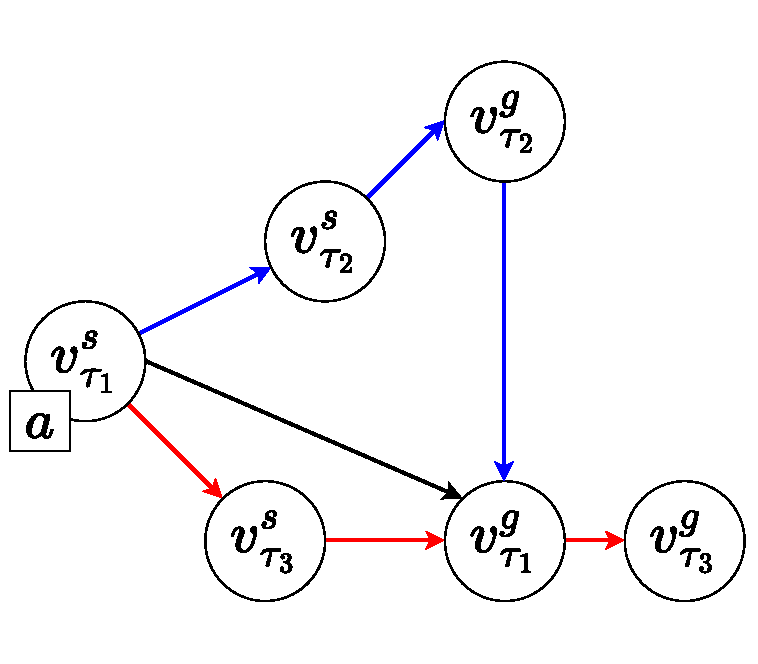
\includegraphics[width=0.5\linewidth]{Fig/carpooling.pdf}
  \caption{The impact of co-passenger tasks}
  \label{fig:carpooling}
  \Description{The impact of co-passenger tasks}
\end{figure}
As shown as in Figure~\ref{fig:carpooling}, there is an agent, $a$, 
and three tasks, $\tau_{1}$, $\tau_{2}$ and $\tau_{3}$.
The agent $a$ is located at pickup location of $\tau_{1}$.
% The black line is the shortest path for agent to complete $\tau_{1}$.
The blue lines are the shortest paths for agent $a$ to complete $\tau_{1}$ and $\tau_{2}$.
The red lines are the shortest paths for agent $a$ to complete $\tau_{1}$ and $\tau_{3}$.
When we allocate $\tau_{1}$ and $\tau_{2}$ to the agent $a$,
the agent $a$ needs to take the blue paths to complete $\tau_{1}$ and $\tau_{2}$ by greedy strategy,
and it will not impact the completion time of $\tau_{2}$ but lengthen the completed time of $\tau_{1}$.
Howerver, if we allocate $\tau_{1}$ and $\tau_{3}$ to the agent $a$, 
$a$ needs to take the red paths to complete $\tau_{1}$ and $\tau_{3}$.
While it also lengthens the completed time of $\tau_{1}$, 
it is obvious that $\tau_3$ has less of an effect on $\tau_1$ as compared to $\tau_{2}$.
Therefore, we need to consider the impact of "co-passenger" tasks when allocating tasks to agents.
We 
\begin{figure}[htbp]
  \centering
  \subfigure[$Path^1_{i,j}$]{
    \label{fig:path1}
    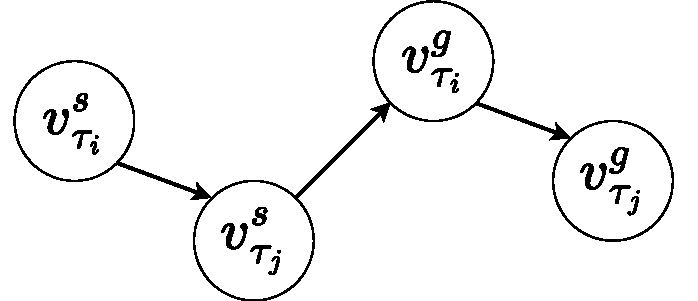
\includegraphics[width=0.4\linewidth]{Fig/path1.pdf}}
  \subfigure[$Path^2_{i,j}$]{
    \label{fig:path2}
    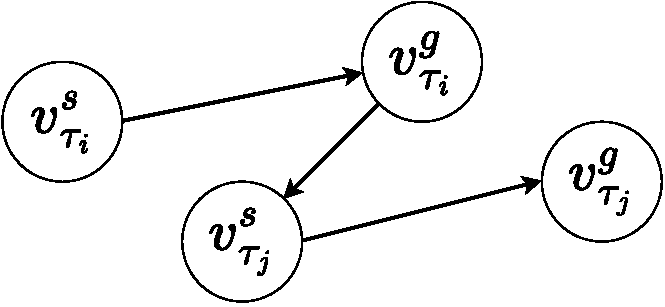
\includegraphics[width=0.4\linewidth]{Fig/path2.pdf}}
  \caption{All possible paths of two tasks}
  \label{fig:2TP}
  \Description{All possible paths of two tasks}
\end{figure}

% We firstly quantify the carpooling chance between two tasks using Equation~(\ref{eq:cp2}).

\begin{eqnarray}
  \label{eq:cp2}
  \Delta_{i,j} = min
\end{eqnarray}



\begin{theorem}
  \label{thm:TaskGroupCost}
  Given a set of tasks $\Gamma_{N}$, 
\end{theorem}

\begin{eqnarray}
\label{eq:tgc}
    Cost \leq \sum_{\tau_i \in \Gamma_N}{dis(v^{s}_{\tau_i}, v^{g}_{\tau_i})} - 2*(N-1)\Delta
\end{eqnarray}

\begin{proof}
    this is a proof.
\end{proof}

\subsection{K-Capacity Hierarchical Clustering}
Based on Theorem~\ref{thm:TaskGroupCost}, we can divide the set of tasks into groups.
The K-Capacity Hierarchical Clustering Algorithm (KCHC) is proposed to divide the set of tasks into groups.
The KCHC algorithm is shown in Algorithm~\ref{alg:KCHC}.

\begin{algorithm}[ht]
\caption{K-Capacity Hierarchical Clustering Algorithm}
\label{alg:KCHC}
\begin{algorithmic}
\REQUIRE $N$ tasks $\Gamma_{N}$, $K$ capacity.
\ENSURE $M$ task groups $\Gamma_{M}$.
\STATE $M \leftarrow 0$
\end{algorithmic}
\end{algorithm}

% \balance

%%%%%%%%%%%%%%%%%%%%%%%%%%%%%%%%%%%%%%%%%%%%%%%%%%%%%%%%%%%%%%%%%%%%%%%%

%%% The acknowledgments section is defined using the "acks" environment
%%% (rather than an unnumbered section). The use of this environment 
%%% ensures the proper identification of the section in the article 
%%% metadata as well as the consistent spelling of the heading.

\begin{acks}
  This work is financially supported by Shenzhen Science and Technology Program 
  under Grant No.GXWD20220817124827001 and No.JCYJ20210324132406016.
\end{acks}

%%%%%%%%%%%%%%%%%%%%%%%%%%%%%%%%%%%%%%%%%%%%%%%%%%%%%%%%%%%%%%%%%%%%%%%%

%%% The next two lines define, first, the bibliography style to be 
%%% applied, and, second, the bibliography file to be used.

\bibliographystyle{ACM-Reference-Format} 
\bibliography{sample}

%%%%%%%%%%%%%%%%%%%%%%%%%%%%%%%%%%%%%%%%%%%%%%%%%%%%%%%%%%%%%%%%%%%%%%%%

\end{document}

%%%%%%%%%%%%%%%%%%%%%%%%%%%%%%%%%%%%%%%%%%%%%%%%%%%%%%%%%%%%%%%%%%%%%%%%

